\documentclass[journal,12pt,twocolumn]{IEEEtran}
%

\usepackage{setspace}
\usepackage{gensymb}
\singlespacing

\usepackage{amsmath}
\usepackage{amsthm}
\usepackage{txfonts}
\usepackage{cite}
\usepackage{enumitem}
\usepackage{mathtools}
\usepackage{listings}
    \usepackage{color}                                            %%
    \usepackage{array}                                            %%
    \usepackage{longtable}                                        %%
    \usepackage{calc}                                             %%
    \usepackage{multirow}                                         %%
    \usepackage{hhline}                                           %%
    \usepackage{ifthen}                                           %%
  %optionally (for landscape tables embedded in another document): %%
    \usepackage{lscape}     
\usepackage{multicol}
\usepackage{chngcntr}
\renewcommand\thesection{\arabic{section}}
\renewcommand\thesubsection{\thesection.\arabic{subsection}}
\renewcommand\thesubsubsection{\thesubsection.\arabic{subsubsection}}

\renewcommand\thesectiondis{\arabic{section}}
\renewcommand\thesubsectiondis{\thesectiondis.\arabic{subsection}}
\renewcommand\thesubsubsectiondis{\thesubsectiondis.\arabic{subsubsection}}

% correct bad hyphenation here
\hyphenation{op-tical net-works semi-conduc-tor}
\def\inputGnumericTable{}                                 %%

\lstset{
%language=C,
frame=single, 
breaklines=true,
columns=fullflexible
}

\begin{document}
%


\newtheorem{theorem}{Theorem}[section]
\newtheorem{problem}{Problem}
\newtheorem{proposition}{Proposition}[section]
\newtheorem{lemma}{Lemma}[section]
\newtheorem{corollary}[theorem]{Corollary}
\newtheorem{example}{Example}[section]
\newtheorem{definition}[problem]{Definition}
\newcommand{\BEQA}{\begin{eqnarray}}
\newcommand{\EEQA}{\end{eqnarray}}
\newcommand{\define}{\stackrel{\triangle}{=}}

\bibliographystyle{IEEEtran}


\providecommand{\mbf}{\mathbf}
\providecommand{\pr}[1]{\ensuremath{\Pr\left(#1\right)}}
\providecommand{\qfunc}[1]{\ensuremath{Q\left(#1\right)}}
\providecommand{\sbrak}[1]{\ensuremath{{}\left[#1\right]}}
\providecommand{\lsbrak}[1]{\ensuremath{{}\left[#1\right.}}
\providecommand{\rsbrak}[1]{\ensuremath{{}\left.#1\right]}}
\providecommand{\brak}[1]{\ensuremath{\left(#1\right)}}
\providecommand{\lbrak}[1]{\ensuremath{\left(#1\right.}}
\providecommand{\rbrak}[1]{\ensuremath{\left.#1\right)}}
\providecommand{\cbrak}[1]{\ensuremath{\left\{#1\right\}}}
\providecommand{\lcbrak}[1]{\ensuremath{\left\{#1\right.}}
\providecommand{\rcbrak}[1]{\ensuremath{\left.#1\right\}}}
\theoremstyle{remark}
\newtheorem{rem}{Remark}
\newcommand{\sgn}{\mathop{\mathrm{sgn}}}
\providecommand{\abs}[1]{\left\vert#1\right\vert}
\providecommand{\res}[1]{\Res\displaylimits_{#1}} 
\providecommand{\norm}[1]{\left\lVert#1\right\rVert}
\providecommand{\mtx}[1]{\mathbf{#1}}
\providecommand{\mean}[1]{E\left[ #1 \right]}
\providecommand{\fourier}{\overset{\mathcal{F}}{ \rightleftharpoons}}
\providecommand{\system}{\overset{\mathcal{H}}{ \longleftrightarrow}}
\newcommand{\solution}{\noindent \textbf{Solution: }}
\newcommand{\cosec}{\,\text{cosec}\,}
\providecommand{\dec}[2]{\ensuremath{\overset{#1}{\underset{#2}{\gtrless}}}}
\newcommand{\myvec}[1]{\ensuremath{\begin{pmatrix}#1\end{pmatrix}}}
\newcommand{\cmyvec}[1]{\ensuremath{\begin{pmatrix*}[c]#1\end{pmatrix*}}}
\newcommand{\mydet}[1]{\ensuremath{\begin{vmatrix}#1\end{vmatrix}}}
\newcommand{\proj}[2]{\textbf{proj}_{\vec{#1}}\vec{#2}}

\let\StandardTheFigure\thefigure
\let\vec\mathbf


\title{
Linear Algebra and Matrices
}
\author{ G V V Sharma$^{*}$% <-this % stops a space
	\thanks{*The author is with the Department
		of Electrical Engineering, Indian Institute of Technology, Hyderabad
		502285 India e-mail:  gadepall@iith.ac.in. All content in this manual is released under GNU GPL.  Free and open source.}
	
}	




\maketitle


\renewcommand{\thefigure}{\theenumi}
\renewcommand{\thetable}{\theenumi}


\begin{abstract}
This document provides a beginner's latex template for math.
\end{abstract}

\section{Points and Vectors}
\renewcommand{\theequation}{\theenumi}
\begin{enumerate}[label=\thesection.\arabic*.,ref=\thesection.\theenumi]
\numberwithin{equation}{enumi}


\item Name the type of quadrilateral formed, if any, by the following points, and give reasons for your answer.
\begin{align}
\vec{P} = \myvec{-1\\-2}, \vec{Q} =\myvec{1\\0},
\vec{R} =\myvec{-1\\2}, \vec{S} =\myvec{-3\\0}
\end{align}
\solution
In Fig. 	\ref{fig:3.5.4_quadrilateral1}
\begin{align}
\label{eq:constr_vectors_quad1_PSQR}
 \vec{P} - \vec{S} &= 
 \vec{Q} - \vec{R} = \myvec{2\\-2}
\\
\vec {R} - \vec {S} &=
 \vec {Q} - \vec {P} = \myvec{2\\2}
\label{eq:constr_vectors_quad1_RSQP}
\end{align}
%
Hence $PQRS$ is a $\parallel$gm $\because$  opposite sides are parallel. Also, 
\begin{align}
\norm{ \vec{P} - \vec{S}} &= 
\norm{ \vec{Q} - \vec{R}} 
\\
=\norm{\vec {R} - \vec {S}} &=
\norm{ \vec {Q} - \vec {P}} = 2\sqrt{2}
\end{align}
%
$\because$ all sides are equal, the $\parallel$gm is a rhombus. The angle between $PS$ and
$RS$ is given by 
\begin{align}
\cos \theta = \frac{\brak{\vec{S}-\vec{P}}^{\top}\brak{\vec{S}-\vec{R}}}{\norm{\vec{S}-\vec{P}}^{\top}\norm{\vec{S}-\vec{R}}}
\end{align}
%
$\because $
\begin{align}
\brak{\vec{S}-\vec{P}}^{\top}\brak{\vec{S}-\vec{R}} = \myvec{2 & -2}\myvec{2\\2} = 0
\end{align}
upon substituting from \eqref{eq:constr_vectors_quad1_PSQR} and \eqref{eq:constr_vectors_quad1_RSQP}, 
\begin{align}
\cos \theta = 0 \implies PS \perp RS
\end{align}
%
Thus, the rhombus is actually a square.

\begin{figure}[!ht]
	\centering
	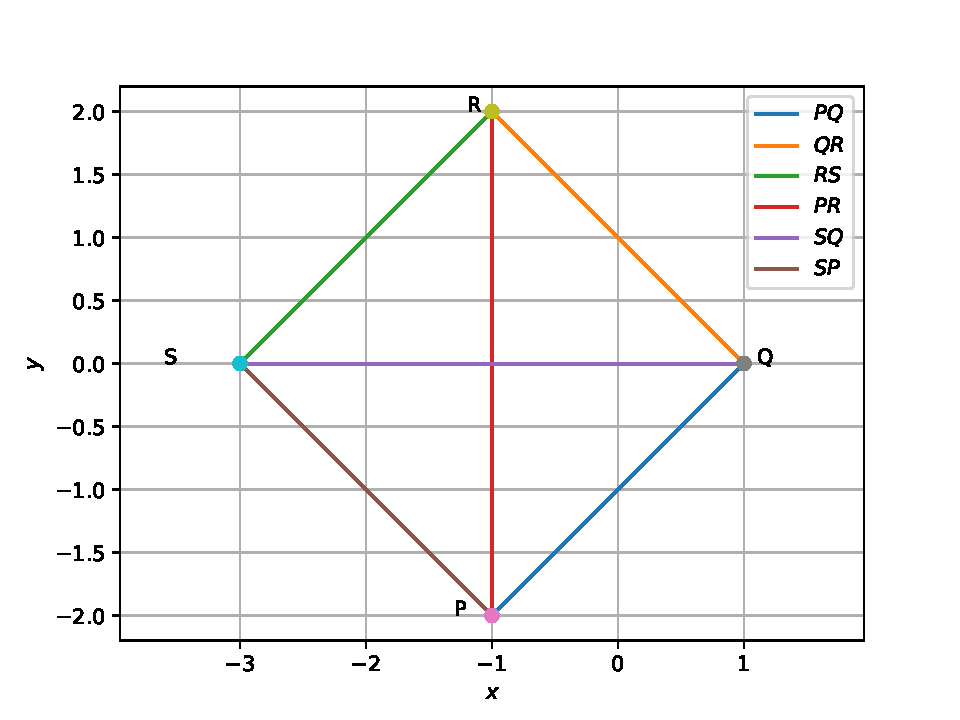
\includegraphics[width=\columnwidth]{quad1.pdf}
	\caption{The given points form a square}
	\label{fig:3.5.4_quadrilateral1}
\end{figure}


\end{enumerate}

\end{document}


